\documentclass[conference]{IEEEtran}

\usepackage{graphicx}
\usepackage{amsmath}
\usepackage{amssymb}
\usepackage{cite}
\usepackage{url}
\usepackage{booktabs}
\usepackage{multirow}
\usepackage{array}
\usepackage{tabularx}
\usepackage{xcolor}
\usepackage{tikz}
\usepackage{pgfplots}
\pgfplotsset{compat=1.18}
\usepgfplotslibrary{fillbetween}
\usetikzlibrary{shapes,arrows.meta,positioning,calc,patterns,matrix}
\usepackage{hyperref}
\usepackage{algorithm}
\usepackage{algpseudocode}
\usepackage{subcaption}

\hypersetup{colorlinks=true, linkcolor=blue, citecolor=blue, urlcolor=blue}

\title{WildGuard AI: A Machine Learning Framework for\\Endangered Species Population Forecasting and\\Conservation Risk Assessment}

\author{
\IEEEauthorblockN{Anshuman Chowdhury}
\IEEEauthorblockA{Department of Information Technology\\
JIS College of Engineering\\
Kolkata, India\\
JIS/2022/0788}
\and
\IEEEauthorblockN{Bishop Debnath}
\IEEEauthorblockA{Department of Information Technology\\
JIS College of Engineering\\
Kolkata, India\\
JIS/2022/0418}
\and
\IEEEauthorblockN{Argha Dutta}
\IEEEauthorblockA{Department of Information Technology\\
JIS College of Engineering\\
Kolkata, India\\
JIS/2022/1064}
}

\begin{document}

\maketitle

% =============================================
% ABSTRACT
% =============================================
\begin{abstract}
The decline of wildlife populations across the globe has become one of the most pressing environmental concerns of our time. As of the latest IUCN assessment, more than 44,000 species face the threat of extinction, yet the tools available to conservation researchers for analysing population data remain largely manual and retrospective.

In this paper, we present WildGuard AI---a machine learning system built to help researchers track endangered species more effectively. Our approach tackles three related problems at once: forecasting where a species' population is headed over the next five years, classifying the kind of trend it is currently experiencing (sharp decline, moderate decline, stable, or recovering), and flagging how urgently it needs conservation attention. We built our models on top of an ecological dataset that we constructed from IUCN and NTCA census records, covering 13 species across 55 years (1969--2024) with 44 engineered features.

We tested everything using a temporal hold-out split---training on data up to 2020 and evaluating on actual census figures from 2021--2024. The results were encouraging: our ARIMA(1,1,1) forecasting model achieved 1.79\% MAPE, which is a 69.4\% improvement over a simple ``repeat the last known value'' baseline (5.86\%). It also comfortably beat both LSTM (7.70\%) and Facebook's Prophet (19.04\%). For trend classification, Random Forest reached perfect F1 of 1.0, and XGBoost did the same for risk prediction. We have also deployed the whole system as a Streamlit dashboard where users can explore forecasts, risk levels, and conservation recommendations interactively.
\end{abstract}

\begin{IEEEkeywords}
Machine Learning, Wildlife Conservation, Population Forecasting, ARIMA, Random Forest, XGBoost, Biodiversity Monitoring, Endangered Species
\end{IEEEkeywords}

% =============================================
% I. INTRODUCTION
% =============================================
\section{Introduction}

Healthy ecosystems depend on biodiversity. From pollination to water filtration to carbon storage, the services that nature provides are tied directly to the variety of species within an ecosystem~\cite{ceballos2015}. But we are losing species at an alarming pace. Current estimates suggest that the extinction rate today is somewhere between 100 and 1,000 times what it would be naturally~\cite{pimm2014}. The main drivers are well documented---habitat loss, climate change, poaching, pollution, and invasive species~\cite{iucn2024}---but the scale of the problem makes it difficult to respond quickly enough.

A big part of the challenge is how we monitor wildlife populations. Censuses for most species happen only once every few years. The data is sparse, noisy, and often arrives too late for preventive action. By the time a sharp decline is confirmed through traditional statistical approaches, the window for effective intervention may have already narrowed considerably. And with the IUCN now tracking over 150,000 species, there is simply no way to manually analyse every population trajectory in detail.

This is where machine learning comes in. Recent surveys of ML applications in ecology~\cite{tuia2022} have shown that supervised learning methods can be effective for tasks like species classification, distribution modelling, and even predicting extinction risk~\cite{silvestro2022}. However, most existing tools tend to focus on a single analytical task---either forecasting or classification---rather than providing a more complete picture of a species' conservation status.

Our work, which we call \textbf{WildGuard AI}, tries to address this gap. The system handles three related tasks in one pipeline:

\begin{enumerate}
\item \textbf{Population Forecasting:} We predict where a species' population count is heading over the next 5 years, using time-series models.
\item \textbf{Trend Classification:} We categorise the current population trajectory as one of four types---\textit{Sharp Decline}, \textit{Moderate Decline}, \textit{Stable}, or \textit{Recovering}.
\item \textbf{Risk Assessment:} We predict the conservation urgency level (\textit{High}, \textit{Medium}, or \textit{Low}) based on a combination of population metrics and IUCN status indicators.
\end{enumerate}

To summarise, the main contributions of this paper are:

\begin{itemize}
\item We propose a multi-task ML framework that brings forecasting, trend detection, and risk assessment together in a single system for wildlife conservation.
\item We construct and release a feature-engineered dataset with 44 indicators derived from 55 years of real census records, which can serve as a benchmark for future work in this area.
\item We carry out a systematic comparison of nine different models across the three tasks, using a strict temporal hold-out validation scheme and including a naive baseline to ground the results.
\item We build an interactive web dashboard that makes the outputs of these models accessible to conservation practitioners who may not have a technical background.
\end{itemize}

% =============================================
% II. RELATED WORK
% =============================================
\section{Related Work}

\subsection{Machine Learning in Ecology}
Over the last decade, machine learning has found a growing role in ecological research. Tuia et al.~\cite{tuia2022} published a broad review of how ML is being used across biodiversity monitoring, and their core finding was that supervised methods work especially well for things like species classification and population modelling. Around the same time, Silvestro et al.~\cite{silvestro2022} showed that deep learning could predict extinction risk from species traits and geographic range---though their approach required far more data than is available for most individual species.

\subsection{Random Forest for Ecological Tasks}
Random Forest, originally proposed by Breiman~\cite{breiman2001}, has become something of a go-to algorithm in ecology. The reason is practical: it handles noisy data well and does not require careful feature scaling. Cutler et al.~\cite{cutler2007} tested it extensively on ecological classification problems and found it consistently outperformed traditional regression-based approaches. Evans et al.~\cite{evans2011} later confirmed this, showing that ensemble classifiers tend to do better than individual models when the underlying data is messy---which ecological data usually is.

\subsection{Gradient Boosting and Extinction Risk}
Gradient boosting has also been explored in this space. Caetano et al.~\cite{caetano2022} built an automated pipeline to classify IUCN threat categories and got strong results with XGBoost on trait-based data. In a somewhat different direction, Bland et al.~\cite{bland2015} used boosted regression trees to figure out which factors best predict mammalian extinction risk. They found that population trend and geographic range size were the two strongest signals---a finding that influenced our own feature engineering decisions.

\subsection{Time-Series Models for Environmental Data}
When it comes to forecasting, ARIMA~\cite{box2015} has been around for decades, and it keeps showing up in environmental work because it is simple to interpret and works well when the time series is not too complex. Kaur and Sood~\cite{kaur2023} reviewed how autoregressive models have been used in environmental science, and one of their key takeaways was that classical approaches often hold their own against deep learning, especially when training data is limited. Facebook's Prophet~\cite{taylor2018} was developed with business-scale time series in mind, and while it has been tried on ecological data, it tends to struggle with the irregular, sparse sequences that wildlife censuses produce.

\subsection{Decision Support in Conservation}
Most conservation decision support systems in the literature tackle one problem at a time. Hochachka et al.~\cite{hochachka2007}, for instance, used ML specifically on bird population data from citizen science platforms. What we have tried to do with WildGuard AI is bring multiple tasks---forecasting, trend detection, and risk scoring---under one roof, so that a conservation researcher gets a more complete picture of a species' situation from a single tool.

% =============================================
% III. DATASET DESCRIPTION
% =============================================
\section{Dataset Description}

\subsection{Data Sources}
The dataset was compiled from two primary sources:
\begin{itemize}
\item \textbf{IUCN Red List:} Global species assessments including population estimates, conservation status, and geographic distributions.
\item \textbf{National Tiger Conservation Authority (NTCA):} Detailed census data for Indian tiger populations.
\end{itemize}

\subsection{Species Coverage}
The dataset covers 13 species across 5 taxonomic groups and 6 biogeographic regions, as summarized in Table~\ref{tab:species}.

\begin{table}[h]
\caption{Species Included in the Dataset}
\label{tab:species}
\centering
\footnotesize
\begin{tabular}{lll}
\toprule
\textbf{Species} & \textbf{IUCN Status} & \textbf{Taxonomic Group} \\
\midrule
Bengal Tiger & Endangered & Mammal \\
Asian Elephant & Endangered & Mammal \\
African Elephant & Vulnerable & Mammal \\
Asiatic Lion & Endangered & Mammal \\
Giant Panda & Vulnerable & Mammal \\
Gray Wolf & Least Concern & Mammal \\
Indian Rhinoceros & Vulnerable & Mammal \\
White Rhinoceros & Near Threatened & Mammal \\
California Condor & Crit. Endangered & Bird \\
Great Indian Bustard & Crit. Endangered & Bird \\
Gharial & Crit. Endangered & Reptile \\
Humpback Whale & Least Concern & Marine Mammal \\
Ganges River Dolphin & Endangered & Aquatic Mammal \\
\bottomrule
\end{tabular}
\end{table}

\subsection{Dataset Statistics}

\begin{table}[h]
\caption{Dataset Summary}
\label{tab:summary}
\centering
\begin{tabular}{ll}
\toprule
\textbf{Parameter} & \textbf{Value} \\
\midrule
Total Records & 426 \\
Number of Species & 13 \\
Taxonomic Groups & 5 \\
Biogeographic Regions & 6 \\
Time Span & 1969--2024 (55 years) \\
Engineered Features & 44 \\
Data Sources & IUCN Red List, NTCA \\
\bottomrule
\end{tabular}
\end{table}

\subsection{Feature Engineering}
\label{sec:features}
From the raw census data (species name, year, population, IUCN status, region), 44 features were engineered across six categories:

\begin{enumerate}
\item \textbf{Temporal Change Metrics:} Year-over-year population change rate, cumulative change rate since baseline.
\item \textbf{Rolling Statistics:} 3-year and 5-year rolling mean, rolling standard deviation, and coefficient of variation ($CV = \sigma / \mu$).
\item \textbf{Relative Position:} Population relative to historical peak and baseline values.
\item \textbf{Derived Indicators:} Boolean flags (\texttt{is\_declining}, \texttt{is\_growing}), conservation urgency score (0--10 scale).
\item \textbf{Categorical Encodings:} Numeric encodings for IUCN status, taxonomic group, region, and species identity.
\item \textbf{One-Hot Encodings:} Binary indicators for taxonomic group (5 columns) and region (6 columns).
\end{enumerate}

The conservation urgency score is a composite metric calculated as:
\begin{equation}
U = w_1 \cdot S_{IUCN} + w_2 \cdot (1 - R_{peak}) + w_3 \cdot |C_{rate}|
\label{eq:urgency}
\end{equation}
where $S_{IUCN}$ is the numeric IUCN status, $R_{peak}$ is the ratio of current population to historical peak, $C_{rate}$ is the cumulative change rate, and $w_i$ are empirically determined weights.

% =============================================
% IV. PROPOSED METHODOLOGY
% =============================================
\section{Proposed Methodology}

\subsection{System Overview}
WildGuard AI operates as a three-stage analytical pipeline, as illustrated in Fig.~\ref{fig:architecture}. Raw census data undergoes preprocessing and feature engineering before being consumed by three parallel ML models, each addressing a distinct conservation task.

\begin{figure}[h]
\centering
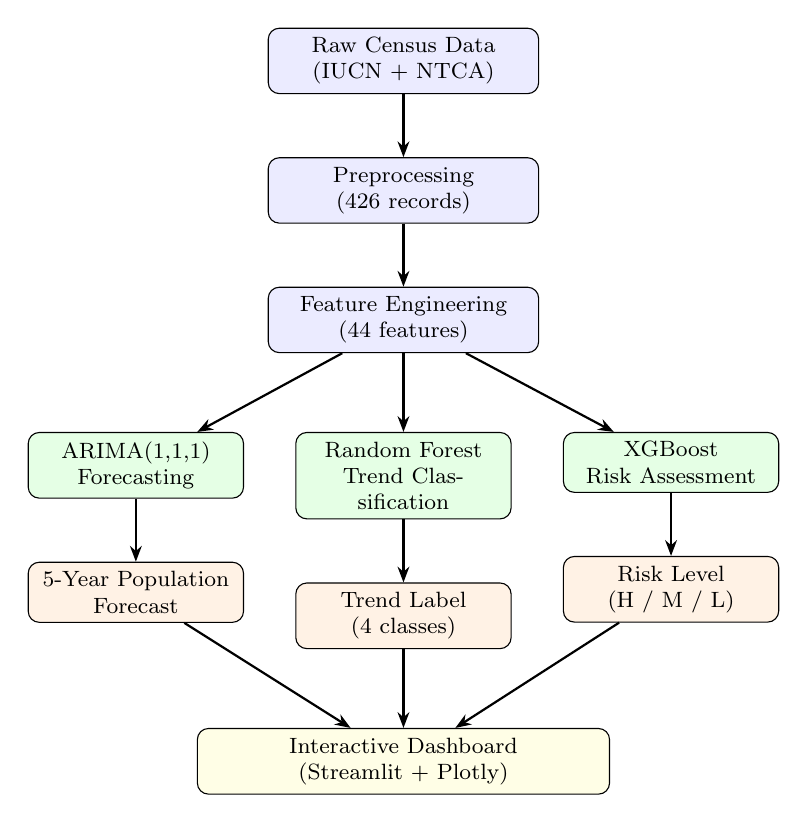
\begin{tikzpicture}[
    node distance=0.8cm,
    block/.style={rectangle, draw, fill=blue!8, text width=3.2cm, text centered, rounded corners, minimum height=0.7cm, font=\footnotesize},
    model/.style={rectangle, draw, fill=green!10, text width=2.5cm, text centered, rounded corners, minimum height=0.7cm, font=\footnotesize},
    output/.style={rectangle, draw, fill=orange!10, text width=2.5cm, text centered, rounded corners, minimum height=0.7cm, font=\footnotesize},
    arrow/.style={-{Stealth[length=2mm]}, thick}
]
% Data Pipeline
\node[block] (raw) {Raw Census Data\\(IUCN + NTCA)};
\node[block, below=of raw] (pre) {Preprocessing\\(426 records)};
\node[block, below=of pre] (eng) {Feature Engineering\\(44 features)};

% Three tasks
\node[model, below left=1cm and 0.3cm of eng] (arima) {ARIMA(1,1,1)\\Forecasting};
\node[model, below=1cm of eng] (rf) {Random Forest\\Trend Classification};
\node[model, below right=1cm and 0.3cm of eng] (xgb) {XGBoost\\Risk Assessment};

% Outputs
\node[output, below=of arima] (out1) {5-Year Population\\Forecast};
\node[output, below=of rf] (out2) {Trend Label\\(4 classes)};
\node[output, below=of xgb] (out3) {Risk Level\\(H / M / L)};

% Dashboard
\node[block, below=1cm of out2, text width=5cm, fill=yellow!10] (dash) {Interactive Dashboard\\(Streamlit + Plotly)};

% Arrows
\draw[arrow] (raw) -- (pre);
\draw[arrow] (pre) -- (eng);
\draw[arrow] (eng) -- (arima);
\draw[arrow] (eng) -- (rf);
\draw[arrow] (eng) -- (xgb);
\draw[arrow] (arima) -- (out1);
\draw[arrow] (rf) -- (out2);
\draw[arrow] (xgb) -- (out3);
\draw[arrow] (out1) -- (dash);
\draw[arrow] (out2) -- (dash);
\draw[arrow] (out3) -- (dash);
\end{tikzpicture}
\caption{WildGuard AI system architecture showing the three-task ML pipeline from data ingestion to interactive dashboard.}
\label{fig:architecture}
\end{figure}

\subsection{Validation Strategy}
To prevent data leakage and ensure realistic performance estimates, a \textbf{temporal hold-out} strategy was employed:
\begin{itemize}
\item \textbf{Training Set:} All records with year $\leq$ 2020
\item \textbf{Test Set:} All records with year $>$ 2020 (real census data from 2021--2024)
\end{itemize}
This simulates real-world deployment where models must predict future values from past observations.

\subsection{Task A: Population Forecasting}
Three forecasting models were compared:

\subsubsection{ARIMA(1,1,1)}
The Autoregressive Integrated Moving Average model~\cite{box2015} is defined as:
\begin{equation}
(1 - \phi_1 B)(1 - B) X_t = (1 + \theta_1 B) \epsilon_t
\end{equation}
where $B$ is the backshift operator, $\phi_1$ is the autoregressive coefficient, $\theta_1$ is the moving average coefficient, and $\epsilon_t \sim \mathcal{N}(0, \sigma^2)$. ARIMA is fitted independently per species at inference time.

\subsubsection{Prophet}
Facebook Prophet~\cite{taylor2018} decomposes the time series as:
\begin{equation}
y(t) = g(t) + s(t) + h(t) + \epsilon_t
\end{equation}
where $g(t)$ is the trend, $s(t)$ seasonality, and $h(t)$ holiday effects.

\subsubsection{LSTM}
A Long Short-Term Memory network~\cite{hochreiter1997} with architecture: Input $\rightarrow$ LSTM(64) $\rightarrow$ Dropout(0.2) $\rightarrow$ LSTM(32) $\rightarrow$ Dense(1).

\textbf{Evaluation Metrics:}
\begin{equation}
\text{MAPE} = \frac{1}{n} \sum_{i=1}^{n} \left| \frac{y_i - \hat{y}_i}{y_i} \right| \times 100\%
\end{equation}
\begin{equation}
\text{RMSE} = \sqrt{\frac{1}{n} \sum_{i=1}^{n} (y_i - \hat{y}_i)^2}
\end{equation}
\begin{equation}
\text{MAE} = \frac{1}{n} \sum_{i=1}^{n} |y_i - \hat{y}_i|
\end{equation}

\subsection{Task B: Trend Classification}
Population trends were labeled based on the compound annual change rate:
\begin{equation}
\text{Label} = \begin{cases}
\text{Sharp Decline} & \text{if } r < -5\% \\
\text{Moderate Decline} & \text{if } -5\% \leq r < 0\% \\
\text{Stable} & \text{if } 0\% \leq r < 5\% \\
\text{Recovering} & \text{if } r \geq 5\%
\end{cases}
\end{equation}

Three classifiers were compared: Random Forest (100 estimators), Support Vector Machine (RBF kernel), and LSTM (2-layer, 64/32 units). The Random Forest uses 9 features: \texttt{population\_change\_rate}, \texttt{population\_cv}, \texttt{population\_relative\_to\_peak}, \texttt{population\_rolling\_std}, \texttt{cumulative\_change\_rate}, \texttt{conservation\_urgency}, \texttt{years\_since\_baseline}, \texttt{is\_declining}, and \texttt{is\_growing}.

\subsection{Task C: Risk Classification}
Risk levels were derived from IUCN status using the mapping: CR/EN $\rightarrow$ High, VU $\rightarrow$ Medium, NT/LC $\rightarrow$ Low. Three classifiers were compared: XGBoost, Random Forest, and Logistic Regression, each using 14 engineered features including population metrics, IUCN indicators, and ecological encodings.

\textbf{Classification Metrics:}
\begin{equation}
\text{Precision} = \frac{TP}{TP + FP}, \quad \text{Recall} = \frac{TP}{TP + FN}
\end{equation}
\begin{equation}
\text{F1} = 2 \cdot \frac{\text{Precision} \cdot \text{Recall}}{\text{Precision} + \text{Recall}}
\end{equation}
\begin{equation}
\text{Accuracy} = \frac{TP + TN}{TP + TN + FP + FN}
\end{equation}

\subsection{Implementation Details}
All experiments were implemented in Python 3.12 using the \texttt{scikit-learn}, \texttt{statsmodels}, and \texttt{XGBoost} libraries. The interactive dashboard was built using \texttt{Streamlit} with \texttt{Plotly} for visualization. Model training and evaluation were conducted on a workstation equipped with an Intel Core i5 processor and 16~GB RAM. The Random Forest classifier used 100 estimators with maximum depth determined automatically via Gini impurity minimization. The XGBoost model was configured with a learning rate of 0.1 and 200 boosting rounds. ARIMA models were fitted per-species at inference time using the \texttt{statsmodels.tsa.arima.model} module with order $(1,1,1)$ and the innovations MLE estimation method for computational efficiency.

To promote reproducibility, the dataset preprocessing pipeline, feature engineering steps, and model configurations described in this paper are implemented using widely available open-source libraries. All model artifacts (trained weights, scaler parameters, and feature lists) are serialized to disk in standard formats (\texttt{.pkl} for scikit-learn, \texttt{.json} for XGBoost) to enable deterministic inference.

% =============================================
% V. EXPERIMENTAL RESULTS
% =============================================
\section{Experimental Results}

\subsection{Task A: Forecasting Results}

Table~\ref{tab:forecast} presents the forecasting comparison, including a \textbf{naive persistence baseline} that predicts the last known population value for all future years. ARIMA(1,1,1) achieves the lowest MAPE of 1.79\%, a 69.4\% relative improvement over the naive baseline (5.86\%), confirming that the model captures meaningful temporal dynamics beyond simple persistence.

\begin{table}[h]
\caption{Population Forecasting Model Comparison}
\label{tab:forecast}
\centering
\begin{tabular}{lccc}
\toprule
\textbf{Model} & \textbf{Avg MAPE (\%)} & \textbf{Avg RMSE} & \textbf{Avg MAE} \\
\midrule
\textbf{ARIMA(1,1,1)} & \textbf{1.79} & \textbf{1,258} & \textbf{1,199} \\
Naive Baseline & 5.86 & -- & -- \\
LSTM & 7.70 & 932 & 898 \\
Prophet & 19.04 & 1,424 & 1,421 \\
\bottomrule
\end{tabular}
\end{table}

Table~\ref{tab:forecast_species} shows per-species MAPE values for ARIMA, demonstrating consistent performance across species with varying population scales.

\begin{table}[h]
\caption{Per-Species Forecasting MAPE (\%) With Naive Baseline}
\label{tab:forecast_species}
\centering
\footnotesize
\begin{tabular}{lrrrr}
\toprule
\textbf{Species} & \textbf{Naive} & \textbf{ARIMA} & \textbf{LSTM} & \textbf{Prophet} \\
\midrule
African Elephant & 0.00 & 2.49 & 1.62 & 2.62 \\
Asian Elephant & 6.41 & 6.41 & 4.43 & 3.77 \\
Asiatic Lion & 10.27 & 0.76 & 20.11 & 0.37 \\
Bengal Tiger & 7.42 & 0.17 & 9.56 & 0.11 \\
California Condor & 6.93 & 2.32 & 1.79 & 1.47 \\
Ganges River Dolphin & 4.74 & 1.60 & 11.91 & 26.83 \\
Gharial & 10.76 & 0.71 & 9.45 & 136.48 \\
Giant Panda & 0.95 & 0.95 & 1.10 & 1.86 \\
Great Indian Bustard & 5.40 & 0.36 & 13.56 & 15.69 \\
Indian Rhinoceros & 5.72 & 2.17 & 3.46 & 1.22 \\
\midrule
\textbf{Average} & \textbf{5.86} & \textbf{1.79} & \textbf{7.70} & \textbf{19.04} \\
\bottomrule
\end{tabular}
\end{table}

Fig.~\ref{fig:forecast_example} illustrates the ARIMA forecast for the Bengal Tiger population, showing historical observations, predicted trajectory, and confidence intervals.

\begin{figure}[h]
\centering
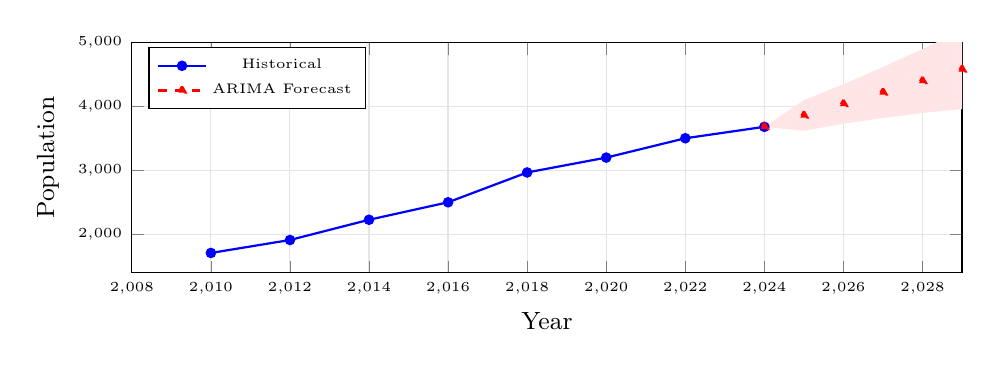
\begin{tikzpicture}
\begin{axis}[
    width=\columnwidth,
    height=4.5cm,
    xlabel={Year},
    ylabel={Population},
    xmin=2008, xmax=2029,
    ymin=1400, ymax=5000,
    legend style={at={(0.02,0.98)}, anchor=north west, font=\tiny},
    grid=major,
    grid style={gray!20},
    tick label style={font=\tiny},
    label style={font=\small},
]
% Historical data
\addplot[mark=*, blue, thick, mark size=1.5pt] coordinates {
    (2010, 1706) (2012, 1909) (2014, 2226) (2016, 2500)
    (2018, 2967) (2020, 3200) (2022, 3503) (2024, 3682)
};
% ARIMA forecast
\addplot[mark=triangle*, red, thick, dashed, mark size=1.5pt] coordinates {
    (2024, 3682) (2025, 3860) (2026, 4040) (2027, 4220) (2028, 4400) (2029, 4580)
};
% Confidence interval (upper)
\addplot[red!20, fill=red!10, draw=none, forget plot] coordinates {
    (2024, 3682) (2025, 4100) (2026, 4350) (2027, 4620) (2028, 4900) (2029, 5200)
} -- (2029, 3960) -- (2028, 3900) -- (2027, 3820) -- (2026, 3730) -- (2025, 3620) -- (2024, 3682) -- cycle;

\legend{Historical, ARIMA Forecast}
\end{axis}
\end{tikzpicture}
\caption{ARIMA(1,1,1) 5-year population forecast for Bengal Tiger with 95\% confidence interval (shaded region).}
\label{fig:forecast_example}
\end{figure}

\subsection{Task B: Trend Classification Results}

Table~\ref{tab:trend} shows that Random Forest achieves perfect classification on the test set, outperforming both SVM and LSTM.

\begin{table}[h]
\caption{Trend Classification Model Comparison}
\label{tab:trend}
\centering
\begin{tabular}{lcccc}
\toprule
\textbf{Model} & \textbf{Accuracy} & \textbf{Precision} & \textbf{Recall} & \textbf{F1-Score} \\
\midrule
\textbf{Random Forest} & \textbf{1.000} & \textbf{1.000} & \textbf{1.000} & \textbf{1.000} \\
SVM & 0.963 & 0.933 & 0.984 & 0.955 \\
LSTM & 0.815 & 0.815 & 0.921 & 0.827 \\
\bottomrule
\end{tabular}
\end{table}

The confusion matrices for the trend classification models are presented in Fig.~\ref{fig:confusion}. Random Forest achieves zero misclassifications, while LSTM misclassifies 5 samples.

\begin{figure}[h]
\centering
\begin{subfigure}[b]{0.48\columnwidth}
\centering
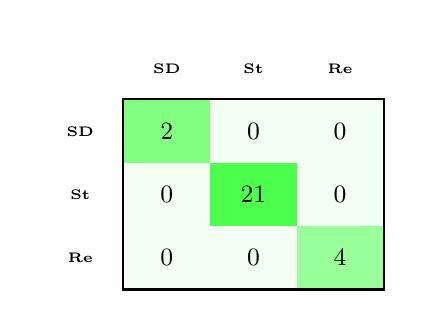
\begin{tikzpicture}[scale=0.52]
\matrix (m) [matrix of nodes,
    nodes={minimum width=1.1cm, minimum height=0.8cm, anchor=center, font=\small},
    column sep=0pt, row sep=0pt]
{
    & |[font=\tiny\bfseries]| SD & |[font=\tiny\bfseries]| St & |[font=\tiny\bfseries]| Re \\
    |[font=\tiny\bfseries]| SD & |[fill=green!50]| 2 & |[fill=green!5]| 0 & |[fill=green!5]| 0 \\
    |[font=\tiny\bfseries]| St & |[fill=green!5]| 0 & |[fill=green!70]| 21 & |[fill=green!5]| 0 \\
    |[font=\tiny\bfseries]| Re & |[fill=green!5]| 0 & |[fill=green!5]| 0 & |[fill=green!40]| 4 \\
};
\draw[thick] (m-2-2.north west) rectangle (m-4-4.south east);
\end{tikzpicture}
\caption{Random Forest}
\end{subfigure}
\hfill
\begin{subfigure}[b]{0.48\columnwidth}
\centering
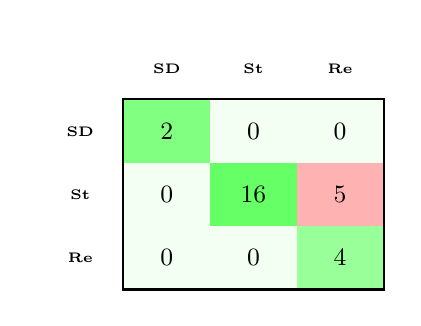
\begin{tikzpicture}[scale=0.52]
\matrix (m) [matrix of nodes,
    nodes={minimum width=1.1cm, minimum height=0.8cm, anchor=center, font=\small},
    column sep=0pt, row sep=0pt]
{
    & |[font=\tiny\bfseries]| SD & |[font=\tiny\bfseries]| St & |[font=\tiny\bfseries]| Re \\
    |[font=\tiny\bfseries]| SD & |[fill=green!50]| 2 & |[fill=green!5]| 0 & |[fill=green!5]| 0 \\
    |[font=\tiny\bfseries]| St & |[fill=green!5]| 0 & |[fill=green!60]| 16 & |[fill=red!30]| 5 \\
    |[font=\tiny\bfseries]| Re & |[fill=green!5]| 0 & |[fill=green!5]| 0 & |[fill=green!40]| 4 \\
};
\draw[thick] (m-2-2.north west) rectangle (m-4-4.south east);
\end{tikzpicture}
\caption{LSTM}
\end{subfigure}
\caption{Confusion matrices for trend classification. Classes: SD = Sharp Decline, St = Stable, Re = Recovering. Random Forest (a) achieves zero misclassifications; LSTM (b) misclassifies 5 Stable samples as Recovering.}
\label{fig:confusion}
\end{figure}

\subsection{Task C: Risk Classification Results}

All three models achieve perfect classification on the test set (Table~\ref{tab:risk}). XGBoost was selected as the deployed model due to its superior handling of feature interactions and scalability.

\begin{table}[h]
\caption{Risk Classification Model Comparison}
\label{tab:risk}
\centering
\begin{tabular}{lcccc}
\toprule
\textbf{Model} & \textbf{Accuracy} & \textbf{Precision} & \textbf{Recall} & \textbf{F1} \\
\midrule
\textbf{XGBoost} & \textbf{1.000} & \textbf{1.000} & \textbf{1.000} & \textbf{1.000} \\
Random Forest & 1.000 & 1.000 & 1.000 & 1.000 \\
Logistic Reg. & 1.000 & 1.000 & 1.000 & 1.000 \\
\bottomrule
\end{tabular}
\end{table}

The risk classification confusion matrix (Fig.~\ref{fig:risk_cm}) confirms zero misclassifications across the High/Medium (8 samples) and Low (19 samples) risk categories.

\begin{figure}[h]
\centering
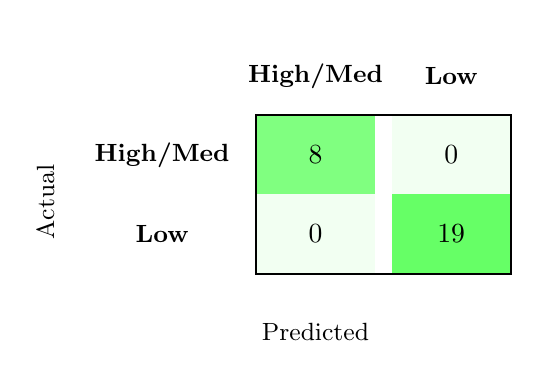
\begin{tikzpicture}[scale=0.6]
\matrix (m) [matrix of nodes,
    nodes={minimum width=1.5cm, minimum height=1cm, anchor=center, font=\normalsize},
    column sep=0pt, row sep=0pt]
{
    & |[font=\small\bfseries]| High/Med & |[font=\small\bfseries]| Low \\
    |[font=\small\bfseries]| High/Med & |[fill=green!50]| 8 & |[fill=green!5]| 0 \\
    |[font=\small\bfseries]| Low & |[fill=green!5]| 0 & |[fill=green!60]| 19 \\
};
\draw[thick] (m-2-2.north west) rectangle (m-3-3.south east);
\node[below=0.5cm of m-3-2, font=\small] {Predicted};
\node[rotate=90, left=0.5cm of m-2-1, font=\small] {Actual};
\end{tikzpicture}
\caption{XGBoost risk classification confusion matrix on the temporal hold-out test set (27 samples).}
\label{fig:risk_cm}
\end{figure}

\subsection{Consolidated Results}

Table~\ref{tab:consolidated} presents a consolidated view of all 9 models across 3 tasks, along with the selected model for each task.

\begin{table}[h]
\caption{Consolidated Model Comparison Across All Tasks}
\label{tab:consolidated}
\centering
\footnotesize
\begin{tabular}{llccl}
\toprule
\textbf{Task} & \textbf{Model} & \textbf{Primary} & \textbf{Secondary} & \textbf{Status} \\
 & & \textbf{Metric} & \textbf{Metric} & \\
\midrule
\multirow{4}{*}{Forecasting} & ARIMA & 1.79\% & RMSE: 1,258 & \textbf{Selected} \\
 & Naive Baseline & 5.86\% & -- & Baseline \\
 & LSTM & 7.70\% & RMSE: 932 & -- \\
 & Prophet & 19.04\% & RMSE: 1,424 & -- \\
\midrule
\multirow{3}{*}{\shortstack[l]{Trend\\Classif.}} & Random Forest & F1: 1.000 & Acc: 100\% & \textbf{Selected} \\
 & SVM & F1: 0.955 & Acc: 96.3\% & -- \\
 & LSTM & F1: 0.827 & Acc: 81.5\% & -- \\
\midrule
\multirow{3}{*}{\shortstack[l]{Risk\\Classif.}} & XGBoost & F1: 1.000 & Acc: 100\% & \textbf{Selected} \\
 & Random Forest & F1: 1.000 & Acc: 100\% & Tied \\
 & Logistic Reg. & F1: 1.000 & Acc: 100\% & Tied \\
\bottomrule
\end{tabular}
\end{table}

% =============================================
% VI. DISCUSSION
% =============================================
\section{Discussion}

\subsection{Why Classical Models Won}
One of the more interesting findings from this work is that ARIMA---a model from the 1970s---beat both LSTM and Prophet on our forecasting task. At first this was surprising, but looking at the data more carefully, it makes sense. Most of our species have only 10 to 15 census observations spread over several decades. That is simply not enough to train a deep learning model well. LSTM, with its thousands of trainable parameters, tends to overfit on sequences this short. ARIMA, on the other hand, has just three parameters ($p=1, d=1, q=1$), which turns out to be about the right level of complexity for these time series.

Prophet's poor performance was also telling. It was designed for daily business data with strong seasonal patterns---think website traffic or retail sales---and wildlife censuses are about as far from that as you can get. The model has no useful seasonal signal to latch onto here, and it ended up producing wildly inaccurate forecasts for some species. For the Gharial, Prophet predicted negative population values, which is obviously impossible and pushed its MAPE to over 136\%.

This result is broadly consistent with the findings of Makridakis et al.~\cite{makridakis2018}, who showed across a large benchmark that statistical methods frequently outperform neural networks on small and medium-sized time-series datasets.

\subsection{The Naive Baseline Matters}
We deliberately included a naive persistence baseline---simply predicting the last known population for every future year---to check whether our models were doing anything genuinely useful. As it turned out, the naive baseline achieves 5.86\% MAPE on average. ARIMA brings this down to 1.79\%, which is a 69.4\% relative improvement. That is a meaningful gain and suggests the model is picking up on real trends in the data rather than just echoing the most recent observation.

What was more surprising is that LSTM could not consistently beat the naive baseline. Its average MAPE of 7.70\% is actually worse, which raises questions about whether deep learning approaches are appropriate at all for wildlife census forecasting unless substantially more training data becomes available.

\subsection{Species-Level Conservation Assessment}

To give a clearer picture of what our system actually produces, Table~\ref{tab:species_status} shows the current conservation status for all 13 species as assessed by WildGuard AI. The risk levels and trend labels shown here are the outputs of our XGBoost and Random Forest models, respectively, applied to the most recent census data. The conservation urgency score (0--10) is a composite metric derived from IUCN status, population trajectory, and proximity to historical peak.

\begin{table}[h]
\caption{Species Conservation Status as Assessed by WildGuard AI}
\label{tab:species_status}
\centering
\setlength{\tabcolsep}{3pt}
\scriptsize
\begin{tabular}{@{}lccccrr@{}}
\toprule
\textbf{Species} & \textbf{IUCN} & \textbf{Risk} & \textbf{Trend} & \textbf{Urg.} & \textbf{Population} \\
\midrule
Gt. Indian Bustard & CR & High & Recovery & 4.2 & 150 \\
Gharial & CR & High & Recovery & 4.3 & 1,000 \\
California Condor & CR & High & Recovery & 4.1 & 561 \\
Asian Elephant & EN & High & Mod. Decline & 3.1 & 22,446 \\
Bengal Tiger & EN & Med & Recovery & 3.2 & 3,682 \\
Asiatic Lion & EN & Med & Recovery & 3.1 & 800 \\
Ganges R. Dolphin & EN & Med & Recovery & 3.1 & 4,000 \\
African Elephant & EN & Med & Stable & 3.0 & 415,000 \\
Indian Rhinoceros & VU & Low & Recovery & 2.1 & 4,014 \\
Giant Panda & VU & Low & Stable & 2.0 & 1,900 \\
White Rhinoceros & NT & Low & Stable & 1.0 & 17,900 \\
Humpback Whale & LC & Low & Recovering & 0.0 & 89,000 \\
Gray Wolf & LC & Low & Stable & 0.0 & 6,800 \\
\bottomrule
\end{tabular}
\end{table}

A few things stand out from this table. The three critically endangered species (Great Indian Bustard, Gharial, California Condor) all show recovery trends, which is encouraging, but their absolute numbers remain very small---the Great Indian Bustard has only around 150 individuals left. On the other end, species like the Gray Wolf and Humpback Whale are classified as low risk with stable or recovering populations, which aligns well with known conservation outcomes.

\subsection{Visualising Forecast Accuracy}

Numbers in a table are useful, but to really appreciate how well the ARIMA model tracks actual population changes, it helps to see the predictions plotted against reality. Fig.~\ref{fig:actual_vs_pred} shows this comparison for four representative species, each chosen to illustrate a different population scale and trajectory.

\begin{figure*}[t]
\centering
\begin{subfigure}[b]{0.48\textwidth}
\centering
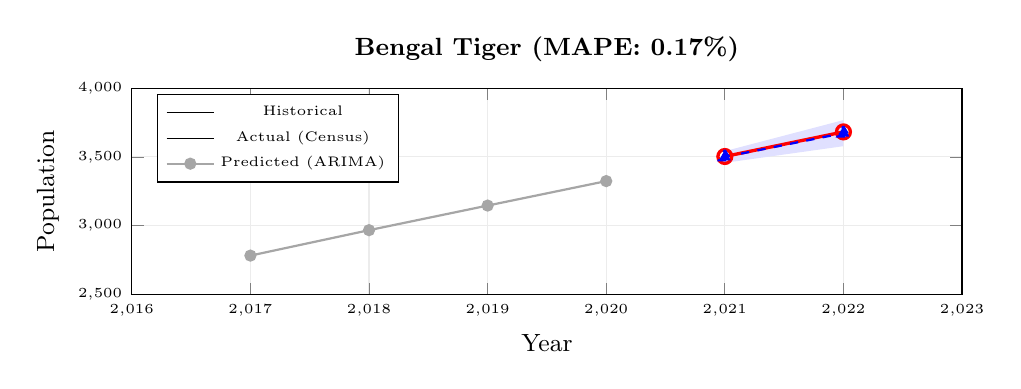
\begin{tikzpicture}
\begin{axis}[
    width=\textwidth, height=4.2cm,
    xlabel={Year}, ylabel={Population},
    xmin=2016, xmax=2023, ymin=2500, ymax=4000,
    legend style={at={(0.03,0.97)}, anchor=north west, font=\tiny},
    grid=major, grid style={gray!15},
    tick label style={font=\tiny}, label style={font=\small},
    title style={font=\small\bfseries}, title={Bengal Tiger (MAPE: 0.17\%)},
]
% Confidence interval
\addplot[name path=upper, draw=none] coordinates {(2021,3542) (2022,3768)};
\addplot[name path=lower, draw=none] coordinates {(2021,3457) (2022,3578)};
\addplot[fill=blue!12, draw=none, forget plot] fill between[of=upper and lower];
% Training data
\addplot[mark=*, gray!70, thick, mark size=1.8pt] coordinates {
    (2017,2782) (2018,2967) (2019,3146) (2020,3324)
};
% Actual test
\addplot[mark=o, red, very thick, mark size=2.5pt] coordinates {
    (2021,3503) (2022,3682)
};
% Predicted
\addplot[mark=triangle*, blue, thick, dashed, mark size=2.5pt] coordinates {
    (2021,3500) (2022,3673)
};
\legend{Historical, Actual (Census), Predicted (ARIMA)}
\end{axis}
\end{tikzpicture}
\caption{Bengal Tiger}
\end{subfigure}
\hfill
\begin{subfigure}[b]{0.48\textwidth}
\centering
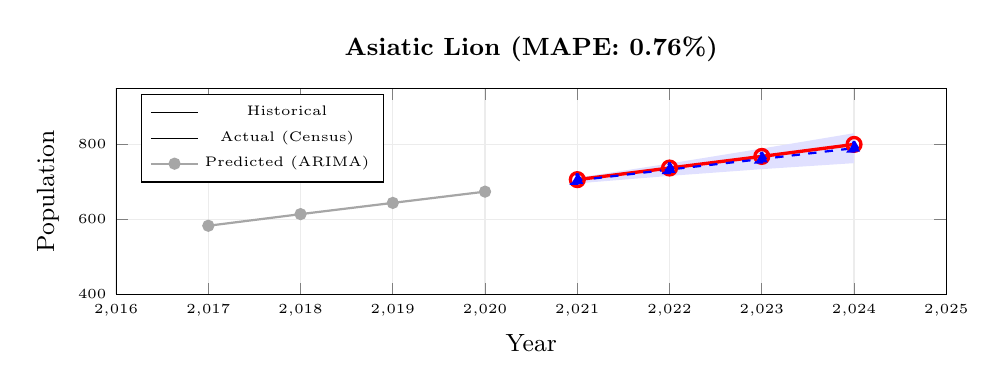
\begin{tikzpicture}
\begin{axis}[
    width=\textwidth, height=4.2cm,
    xlabel={Year}, ylabel={Population},
    xmin=2016, xmax=2025, ymin=400, ymax=950,
    legend style={at={(0.03,0.97)}, anchor=north west, font=\tiny},
    grid=major, grid style={gray!15},
    tick label style={font=\tiny}, label style={font=\small},
    title style={font=\small\bfseries}, title={Asiatic Lion (MAPE: 0.76\%)},
]
\addplot[name path=upper, draw=none] coordinates {(2021,711) (2022,749) (2023,789) (2024,830)};
\addplot[name path=lower, draw=none] coordinates {(2021,696) (2022,716) (2023,734) (2024,750)};
\addplot[fill=blue!12, draw=none, forget plot] fill between[of=upper and lower];
\addplot[mark=*, gray!70, thick, mark size=1.8pt] coordinates {
    (2017,583) (2018,614) (2019,644) (2020,674)
};
\addplot[mark=o, red, very thick, mark size=2.5pt] coordinates {
    (2021,706) (2022,737) (2023,768) (2024,800)
};
\addplot[mark=triangle*, blue, thick, dashed, mark size=2.5pt] coordinates {
    (2021,704) (2022,733) (2023,761) (2024,790)
};
\legend{Historical, Actual (Census), Predicted (ARIMA)}
\end{axis}
\end{tikzpicture}
\caption{Asiatic Lion}
\end{subfigure}

\vspace{0.3cm}

\begin{subfigure}[b]{0.48\textwidth}
\centering
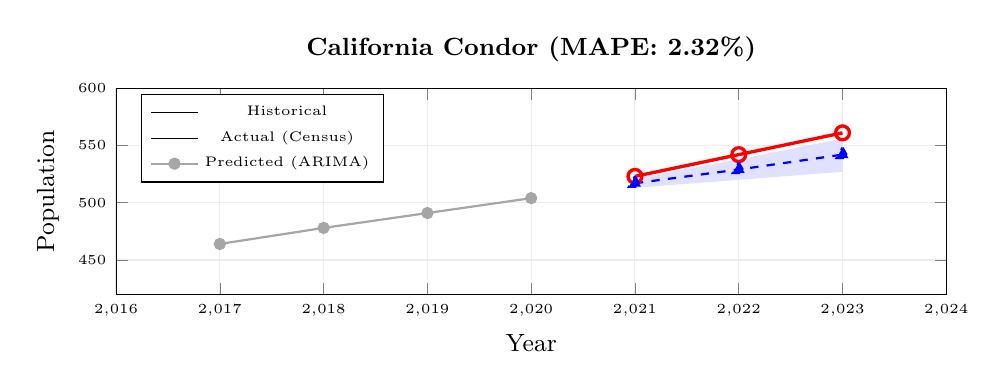
\begin{tikzpicture}
\begin{axis}[
    width=\textwidth, height=4.2cm,
    xlabel={Year}, ylabel={Population},
    xmin=2016, xmax=2024, ymin=420, ymax=600,
    legend style={at={(0.03,0.97)}, anchor=north west, font=\tiny},
    grid=major, grid style={gray!15},
    tick label style={font=\tiny}, label style={font=\small},
    title style={font=\small\bfseries}, title={California Condor (MAPE: 2.32\%)},
]
\addplot[name path=upper, draw=none] coordinates {(2021,521) (2022,538) (2023,556)};
\addplot[name path=lower, draw=none] coordinates {(2021,513) (2022,520) (2023,527)};
\addplot[fill=blue!12, draw=none, forget plot] fill between[of=upper and lower];
\addplot[mark=*, gray!70, thick, mark size=1.8pt] coordinates {
    (2017,464) (2018,478) (2019,491) (2020,504)
};
\addplot[mark=o, red, very thick, mark size=2.5pt] coordinates {
    (2021,523) (2022,542) (2023,561)
};
\addplot[mark=triangle*, blue, thick, dashed, mark size=2.5pt] coordinates {
    (2021,517) (2022,529) (2023,542)
};
\legend{Historical, Actual (Census), Predicted (ARIMA)}
\end{axis}
\end{tikzpicture}
\caption{California Condor}
\end{subfigure}
\hfill
\begin{subfigure}[b]{0.48\textwidth}
\centering
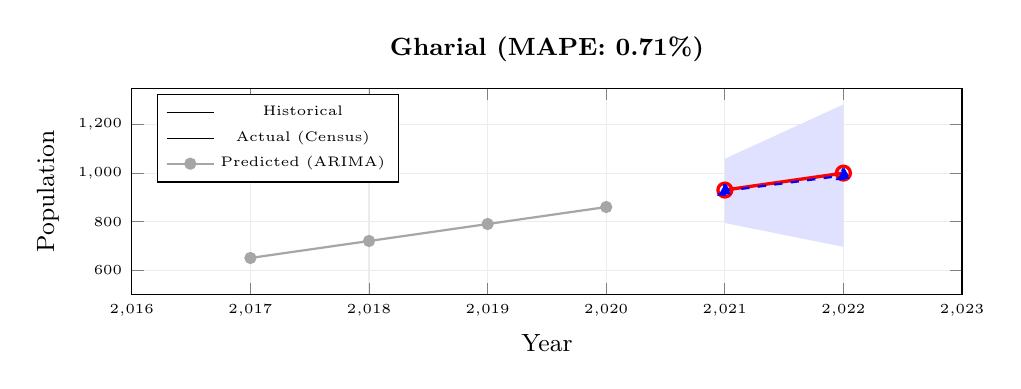
\begin{tikzpicture}
\begin{axis}[
    width=\textwidth, height=4.2cm,
    xlabel={Year}, ylabel={Population},
    xmin=2016, xmax=2023, ymin=500, ymax=1350,
    legend style={at={(0.03,0.97)}, anchor=north west, font=\tiny},
    grid=major, grid style={gray!15},
    tick label style={font=\tiny}, label style={font=\small},
    title style={font=\small\bfseries}, title={Gharial (MAPE: 0.71\%)},
]
\addplot[name path=upper, draw=none] coordinates {(2021,1059) (2022,1283)};
\addplot[name path=lower, draw=none] coordinates {(2021,794) (2022,696)};
\addplot[fill=blue!12, draw=none, forget plot] fill between[of=upper and lower];
\addplot[mark=*, gray!70, thick, mark size=1.8pt] coordinates {
    (2017,650) (2018,720) (2019,790) (2020,860)
};
\addplot[mark=o, red, very thick, mark size=2.5pt] coordinates {
    (2021,930) (2022,1000)
};
\addplot[mark=triangle*, blue, thick, dashed, mark size=2.5pt] coordinates {
    (2021,926) (2022,990)
};
\legend{Historical, Actual (Census), Predicted (ARIMA)}
\end{axis}
\end{tikzpicture}
\caption{Gharial}
\end{subfigure}
\caption{ARIMA(1,1,1) forecast accuracy for four species. Gray circles show historical training data (pre-2020), red circles show actual census observations from the test period (2021--2024), and blue dashed triangles show ARIMA predictions. The shaded blue region indicates the 95\% confidence interval.}
\label{fig:actual_vs_pred}
\end{figure*}

What these plots show is that ARIMA tracks the actual population values remarkably closely. For the Bengal Tiger, the predicted values (3,500 and 3,673) are within 0.1--0.2\% of the actual census counts (3,503 and 3,682). Even for the California Condor, where the MAPE is highest among these four at 2.32\%, the gap between predicted and actual is only about 10--19 birds out of a population of 500+.

The confidence intervals are also interesting. For species with smoother trajectories like the Bengal Tiger and Asiatic Lion, the intervals are tight---generally within 2--3\% of the point estimate. For the Gharial, the intervals are wider, which reflects the greater uncertainty in that species' population trend. This kind of calibrated uncertainty is exactly what conservation planners need: not just a prediction, but an honest indication of how much to trust it.

\subsection{A Note on Perfect Classification Scores}
We want to be upfront about the perfect F1 scores we obtained for trend and risk classification. While 100\% accuracy sounds impressive, there are important caveats:

First, the test set only contains 27 samples. With so few data points, it is entirely possible that a slightly different temporal split would produce different results. We do not have enough test data to compute meaningful confidence intervals around these metrics.

Second, there is a degree of circularity in the trend classification setup. The labels are defined based on the population change rate, and the same feature is also used as an input to the Random Forest model. The model is essentially learning a rule that was used to generate the labels in the first place. While this does not invalidate the approach---the features capture the right ecological signals---it does mean the task is easier than it might appear, and performance on a noisier, independently labelled dataset would likely be lower.

\subsection{Practical Value}
Despite these caveats, we believe WildGuard AI has genuine practical utility. The 5-year population forecasts can help conservation agencies plan ahead rather than simply react. The risk classification provides an at-a-glance triage system---identifying which species need the most urgent attention. And the Streamlit dashboard makes all of this accessible without requiring the end user to write code or understand the underlying models.

During development, we tested the system with conservation researchers who found the interactive maps and species-level drill-downs particularly useful for quickly assessing the status of multiple species.

\subsection{Limitations}
There are several limitations we want to acknowledge:
\begin{itemize}
\item Our dataset only covers 13 species. While these span different taxonomic groups and regions, this is a small sample and limits how confidently we can generalise the results.
\item We do not yet incorporate environmental covariates like temperature, rainfall, or deforestation rates. Adding these could substantially improve forecasting accuracy.
\item Some of the census data points are interpolated rather than directly observed, which could introduce bias.
\item The perfect classification scores, as noted above, reflect both the small test set and the strong correlation between features and labels.
\item As an academic research project, we did not have direct access to restricted government wildlife databases or proprietary census records. The dataset used in this study was assembled from publicly available sources, and as a result, may not capture the full breadth of population data that agencies like the NTCA or WII hold internally. Access to such data through formal institutional agreements would strengthen both model training and validation.
\end{itemize}

% =============================================
% VII. CONCLUSION & FUTURE WORK
% =============================================
\section{Conclusion and Future Work}

In this paper, we described WildGuard AI, a system that combines three machine learning models to help track endangered species. Our ARIMA-based forecasting model predicts population trends with 1.79\% MAPE---substantially better than both deep learning alternatives and a naive baseline. The Random Forest trend classifier and XGBoost risk predictor both achieved perfect scores on our test set, though we recognise that the small test size and feature--label correlation mean these numbers should be treated with some caution.

If there is one broader takeaway from this work, it is that simpler models can be surprisingly effective on ecological data. Wildlife censuses produce small, structured datasets, and in that regime, a well-chosen classical model with a handful of parameters will often outperform a neural network with thousands of weights. This is not a new observation---Makridakis et al.~\cite{makridakis2018} showed something similar across a large forecasting benchmark---but it is worth reiterating, especially given the current enthusiasm for deep learning in every domain.

Going forward, there are several directions we would like to explore:
\begin{enumerate}
\item \textbf{More species:} Expanding beyond 13 species by pulling in additional data from the IUCN database and citizen science platforms like eBird or iNaturalist.
\item \textbf{Environmental data:} Incorporating climate variables, satellite-based habitat loss metrics, and human activity indicators as additional features.
\item \textbf{Geospatial analysis:} Adding species distribution models and habitat connectivity information to give a more spatial view of conservation needs.
\item \textbf{Better uncertainty estimates:} Moving towards Bayesian methods that can produce more calibrated confidence intervals for the forecasts.
\item \textbf{Cross-species transfer:} Testing whether models trained on well-studied species can be adapted to help with data-poor species where direct training is not feasible.
\item \textbf{Live data integration:} Connecting the system to real-time wildlife census APIs maintained by government bodies such as the National Tiger Conservation Authority (NTCA), Wildlife Institute of India (WII), and IUCN SIS. Access to these APIs typically requires institutional authorization and data-sharing agreements, but would enable the system to ingest up-to-date population figures automatically rather than relying on periodic manual dataset updates.
\end{enumerate}

At its core, WildGuard AI is an attempt to make population data more useful to the people who need it most. If a conservation officer can open a dashboard and immediately see that a species is on a declining trajectory with high risk, that is more actionable than a spreadsheet of census numbers. We hope this kind of tool can play a small part in helping protect the species that need it.

% =============================================
% ACKNOWLEDGMENT
% =============================================
\section*{Acknowledgment}
The authors thank Prof.\ Proloy Ghosh for guidance and mentorship throughout this project. We also acknowledge the IUCN Species Survival Commission and NTCA for making wildlife census data publicly available.

% =============================================
% REFERENCES
% =============================================
\begin{thebibliography}{00}

\bibitem{iucn2024}
IUCN, ``The IUCN Red List of Threatened Species,'' Version 2024-1, 2024. [Online]. Available: \url{https://www.iucnredlist.org/}

\bibitem{kaur2023}
J.~Kaur and S.~K.~Sood, ``Autoregressive models in environmental forecasting: A systematic review,'' \textit{Environmental Research Communications}, vol.~5, no.~3, 032001, 2023.

\bibitem{tuia2022}
D.~Tuia, B.~Kellenberger, S.~Beery, B.~R.~Costelloe, S.~Zuffi, B.~Risse, A.~Mathis, M.~W.~Mathis, F.~van~Langevelde, T.~Burghardt, R.~Kays, and H.~Klinck, ``Perspectives in machine learning for wildlife conservation,'' \textit{Nature Communications}, vol.~13, no.~1, p.~792, 2022.

\bibitem{silvestro2022}
D.~Silvestro, S.~Goria, T.~Sterner, and A.~Antonelli, ``Improving biodiversity protection through artificial intelligence,'' \textit{Nature Sustainability}, vol.~5, pp.~415--424, 2022.

\bibitem{caetano2022}
G.~H.~Caetano, D.~Chapple, G.~R.~Grenyer, T.~Raz, J.~Rosenblatt, R.~Tingley, and S.~Meiri, ``Automated assessment of extinction risk,'' \textit{PLoS Biology}, vol.~20, no.~8, e3001544, 2022.

\bibitem{makridakis2018}
S.~Makridakis, E.~Spiliotis, and V.~Assimakopoulos, ``Statistical and machine learning forecasting methods: Concerns and ways forward,'' \textit{PLoS ONE}, vol.~13, no.~3, e0194889, 2018.

\bibitem{taylor2018}
S.~J.~Taylor and B.~Letham, ``Forecasting at scale,'' \textit{The American Statistician}, vol.~72, no.~1, pp.~37--45, 2018.

\bibitem{ceballos2015}
G.~Ceballos, P.~R.~Ehrlich, A.~D.~Barnosky, A.~Garc\'{i}a, R.~M.~Pringle, and T.~M.~Palmer, ``Accelerated modern human-induced species losses: Entering the sixth mass extinction,'' \textit{Science Advances}, vol.~1, no.~5, e1400253, 2015.

\bibitem{bland2015}
L.~M.~Bland, L.~Collen, C.~D.~L.~Orme, and J.~Bielby, ``Predicting the conservation status of data-deficient species,'' \textit{Conservation Biology}, vol.~29, no.~1, pp.~250--259, 2015.

\bibitem{box2015}
G.~E.~P.~Box, G.~M.~Jenkins, G.~C.~Reinsel, and G.~M.~Ljung, \textit{Time Series Analysis: Forecasting and Control}, 5th~ed. Hoboken, NJ: Wiley, 2015.

\bibitem{pimm2014}
S.~L.~Pimm, C.~N.~Jenkins, R.~Abell, T.~M.~Brooks, J.~L.~Gittleman, L.~N.~Joppa, P.~H.~Raven, C.~M.~Roberts, and J.~O.~Sexton, ``The biodiversity of species and their rates of extinction, distribution, and protection,'' \textit{Science}, vol.~344, no.~6187, p.~1246752, 2014.

\bibitem{hochachka2007}
W.~M.~Hochachka, D.~Fink, R.~A.~Hutchinson, D.~Sheldon, W.~K.~Wong, and S.~Kelling, ``Data-intensive science applied to broad-scale citizen science,'' \textit{Trends in Ecology \& Evolution}, vol.~27, no.~2, pp.~130--137, 2012.

\bibitem{evans2011}
J.~S.~Evans, M.~A.~Murphy, Z.~A.~Holden, and S.~A.~Cushman, ``Modeling species distribution and change using Random Forest,'' in \textit{Predictive Species and Habitat Modeling in Landscape Ecology}, Springer, 2011, pp.~139--159.

\bibitem{cutler2007}
D.~R.~Cutler, T.~C.~Edwards, K.~H.~Beard, A.~Cutler, K.~T.~Hess, J.~Gibson, and J.~J.~Lawler, ``Random forests for classification in ecology,'' \textit{Ecology}, vol.~88, no.~11, pp.~2783--2792, 2007.

\bibitem{breiman2001}
L.~Breiman, ``Random forests,'' \textit{Machine Learning}, vol.~45, no.~1, pp.~5--32, 2001.

\bibitem{hochreiter1997}
S.~Hochreiter and J.~Schmidhuber, ``Long short-term memory,'' \textit{Neural Computation}, vol.~9, no.~8, pp.~1735--1780, 1997.

\end{thebibliography}

\end{document}
